%!TEX root = ../main.tex
\chapter{Experiments and Workflow}\label{chap:experiments}
本節では、主に実環境データを対象にした、屈折を考慮した水中3次元再構成のための完全なパイプラインとその実装を概説する。

% \begin{figure}[htbp]
%   \centering
%   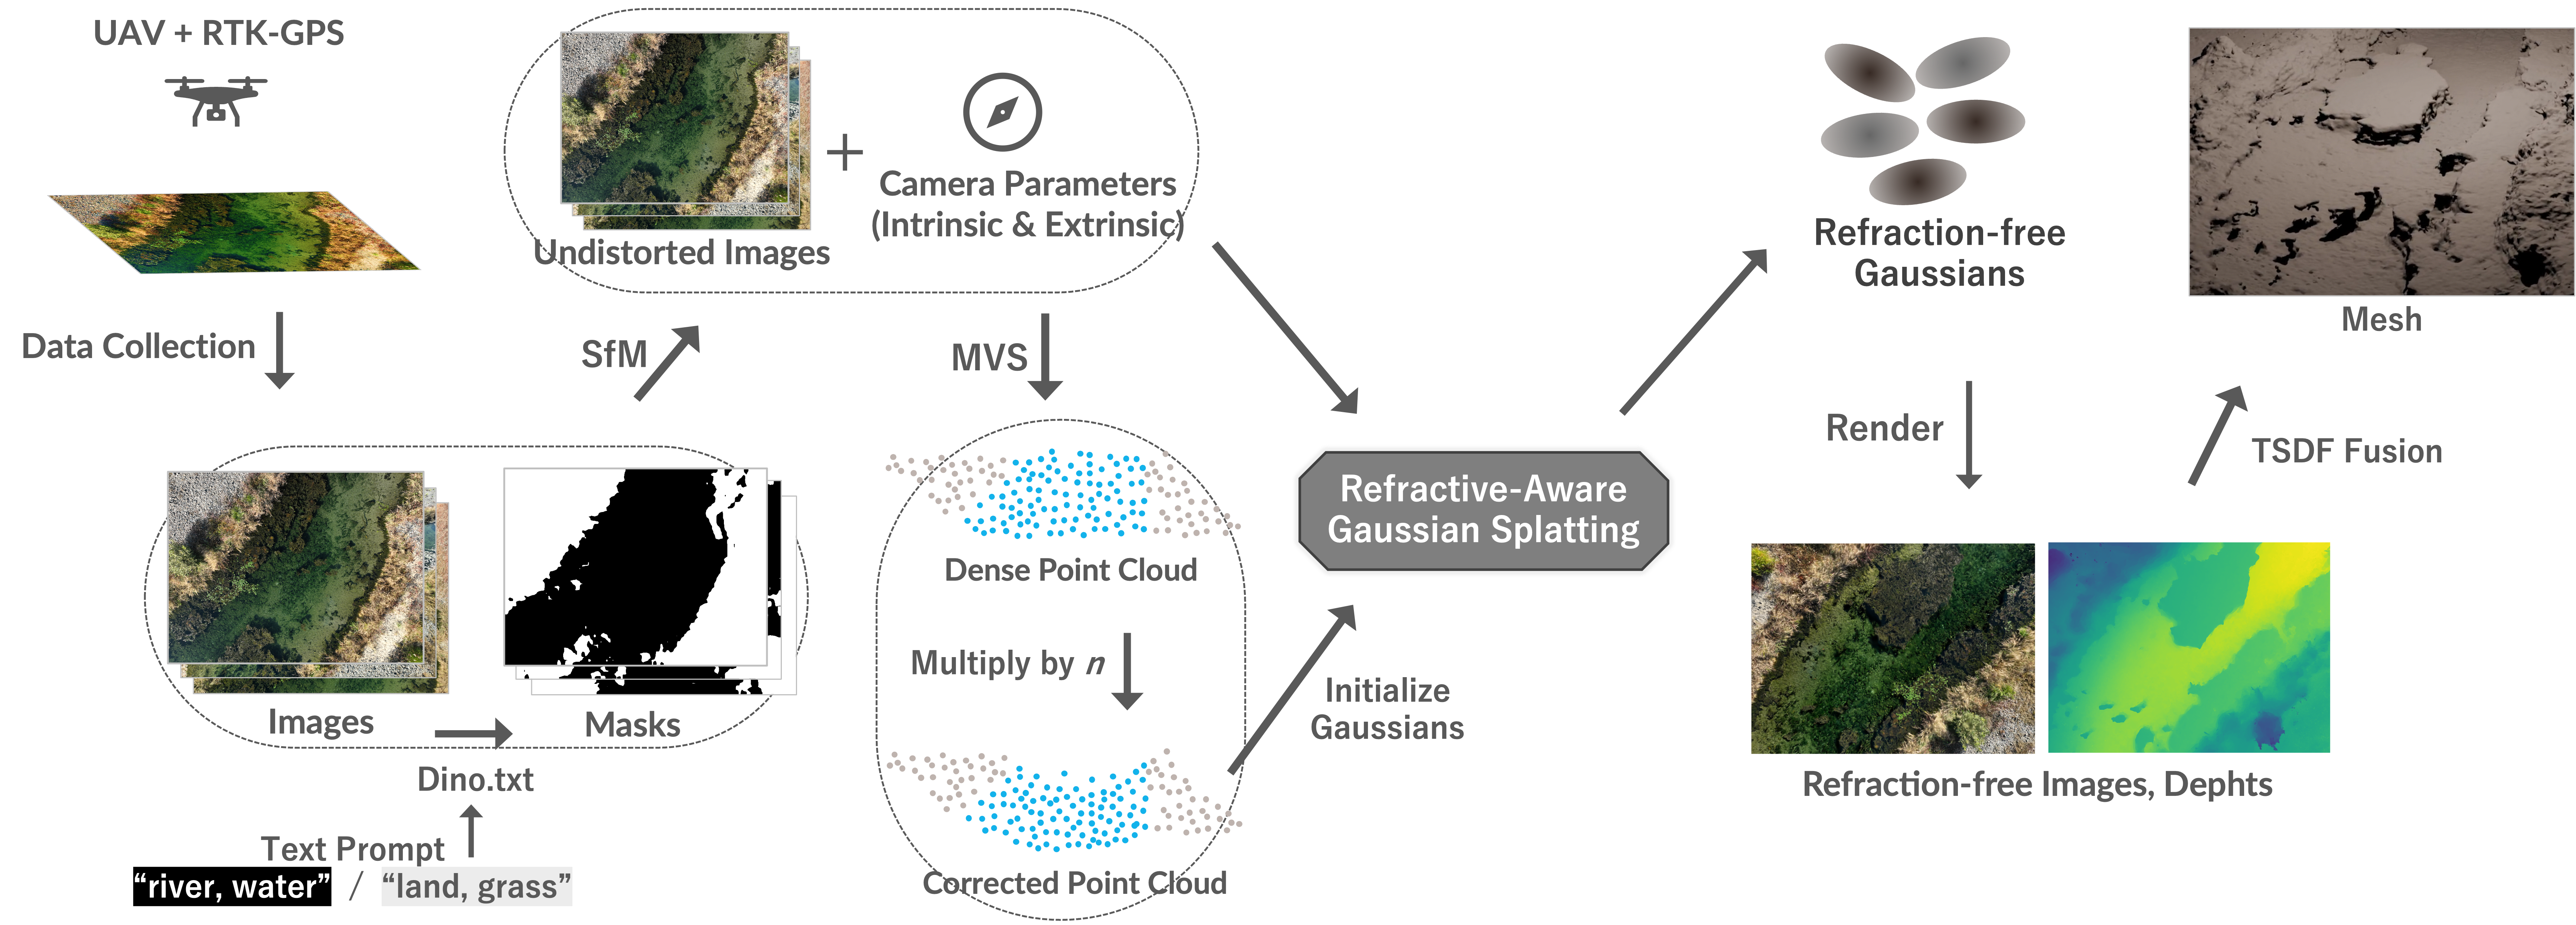
\includegraphics[width=0.95\textwidth]{figure/70_experim/workflow.png}
%   \caption{
%     実環境データを対象にした、屈折を考慮した水中3次元再構成のための完全なパイプライン。
%     }
%     \label{fig:workflow}
% \end{figure}

\begin{sidewaysfigure}[p]
  \centering
  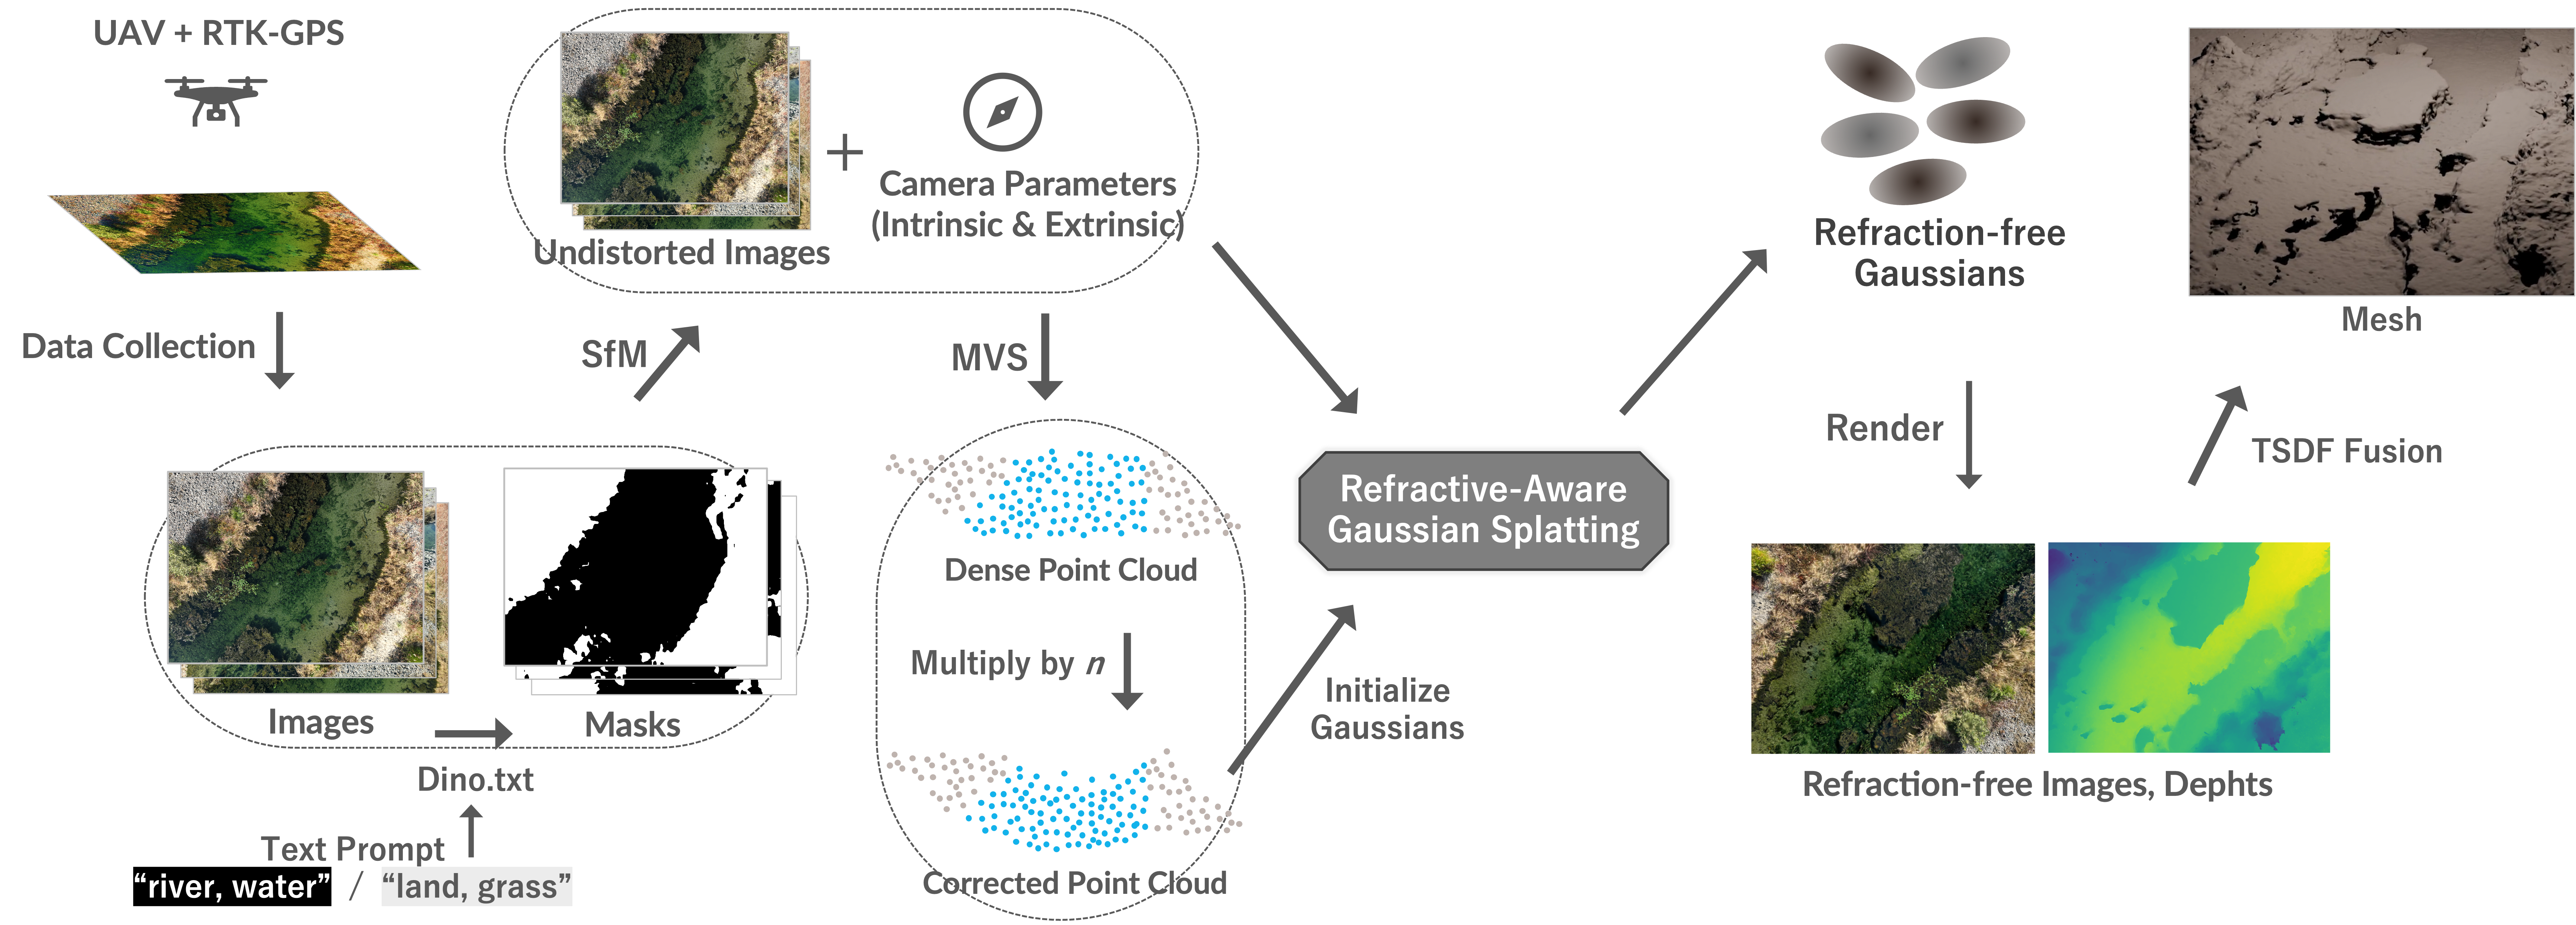
\includegraphics[width=0.95\textheight, keepaspectratio]{figure/70_experim/workflow.png}
  \caption{
    実環境データを対象にした、屈折を考慮した水中3次元再構成のための完全なパイプライン。
    }
  \label{fig:workflow}
\end{sidewaysfigure}

\note{Abstract図表をより詳細に説明する}

\section{Camera Calibration}\label{sec:camera-calibration}

RA-GSは、他の他視点三次元再構成タスク(\cref{subsec:mvs,subsec:nvs})と同様に、正確なカメラ内部・外部パラメータと歪みのない画像(Undistorted Images)を必要とする。
これらは、COLMAP~\cite{schoenberger2016_colmap}などのSfM(\cref{subsec:sfm})によって推定することが標準となっている。
本研究では、学術研究が無料のフォトグラメトリソフトウェアであるRealityScan\cite{RealityScan}を使用し、カメラキャリブレーションと画像の歪み補正を行った。
\cref{sec:field-dataset}で示したように、スケール不定性を持つ多視点画像による再構成に対し、高精度なRTK-GPSの位置情報をリファレンスに用いることで、実環境に即したスケールを保証する。

陸域を十分に撮像できず、後続の水面マスク抽出手法が適用できない場合は、R-SfM\cite{Makris2024_refractive-aware-sfm}を用いて、屈折領域込みでのカメラポーズ推定が可能である。
また、RA-GSでは、カメラ外部パラメータに関しての勾配も追跡可能で、Photometricな情報からのカメラポーズ推定も可能であり、予め使用するカメラの内部キャリブレーションを行っておくことで、ジオリファレンス情報や屈折により誤差の増加したSfMによるカメラ位置姿勢を初期値として、シーンと同時にカメラ姿勢を最適化していくことも可能である。

\section{Mask Generation by Vision-Language Models}\label{sec:mask-generation}

本研究が対象とする空気中から水面下を対象としたシーンにおいては、光の屈折により、
やはりSfMが前提とする光の直進性が成立しなくなり、精度は悪化する
~\cite{she2024IROS_Refractive-COLMAP}。

\cite{she2024IROS_Refractive-COLMAP,Chadebecq2017ICCV_Refractive-Structure-from-Motion,Sedlazeck2013ICCV_Refractive-Structure-from-Motion,Makris2024_refractive-aware-sfm}
など、明示的に屈折を考慮したSfMは提案されているが、RA-GSの性能を最大限正確に検証するため、本研究では水面をマスクすることで、陸域のStaticなSceneのみを用いて特徴点検出から始まるSfMプロセスを行い、正確なカメラパラメータを推定する。
これは、一般のシーンの三次元復元でも一般的な手法であり、陸域であれば、人物や車両などの移動体、鏡などの反射物(Distractor)をマスクとして除外する機能は、RealityScanのみならず、COLMAPや他の商用フォトグラメトリソフトウェアでも同様の手法が実現可能である。
陸域で十分な特徴点を得られるように\cref{sec:field-dataset}で取得したUAV画像には十分な陸域が写っていることを確認した。


UAV画像から水面や Distractor を抽出するマスク生成には、以下のことがらが実務における効率の観点から求められる。

\begin{itemize}
  \item Automated:
    数十〜数百枚規模の UAV 画像に対して、オペレータが1枚ずつ手動ラベリングを行うことは現実的ではなく、
    自動的に大規模な画像データからマスクを生成できる必要がある。
  \item Robustness:
    水底の特性、季節・天候や時間帯によるシーンの変化、陸域・植生など、実フィールドにおける多様なシーンの構成要素に対して安定して頑健に対象のマスクを生成できる必要がある。
  \item Zero-Shot Adaptability:
    自動化を実現するための深層学習モデルに対し、現場ごとに追加のアノテーションや再学習を行うことは、手動ラベリングと同様の多大なコストを要する。
    多様な現場に対して、同一のモデルを適応させることができることが望ましい。
  \item Controllability:
    「water surface」「boat」「people」といった自然言語のプロンプトを用いて、環境内の対象クラスを柔軟に切り替えられることは、
    RobustnessやZero-Shot Adaptabilityの根底にある要件であり、高いインタラクティビティを提供する。
\end{itemize}

本研究では、オープン語彙物体検出モデル(DINO.txt\cite{Jose2025CVPR_DINOv2-Text,Simeoni2025_DINOv3})を採用し、テキストプロンプトによるゼロショット・セグメンテーションを行う。

\begin{figure}[htbp]
  \centering
  \includegraphics[width=0.95\textwidth]{figure/70_experim/DinoTXT.png}
  \caption{
    Dino.txtの概要。
    \cite{Jose2025CVPR_DINOv2-Text}から引用。\\
    (左):DinoV2\cite{Oquab2023_DINOv2}による自己教師あり学習(Self-Supervised Learning: SSL)による特徴量の主成分分析による可視化。
     (本研究では、DinoV3\cite{Simeoni2025_DINOv3}を使用している)
    (中央):学習済SSLと、ゼロから学習したテキストエンコーダを整合させるトレーニング戦略。
    視覚エンコーダ上に軽量なビジョンブロックを追加することで、テキストとの整合性をさらに向上させている。
    モデル全体はわずか5万イテレーションで学習可能であり、ゼロショット分類およびオープン語彙セグメンテーションの両タスクにおいて高い性能を有する。
    (右):出力結果例。(入力画像と、対応する zero-shot分類や open-vocabularyセグメンテーションの結果)。
    }
    \label{fig:DinoTXT}
\end{figure}

\missingfigure{実際のマスク作成例。定量も含めて示す}

本研究の浅水域を対象とした、水域と陸域を区別する。
前章で示した宇治川のデータを例に上げると、水面はマスクにより除外し(0値)、陸域には陸地や草木などが含まれ、それらを非マスクとして残す(1値)。
今回は非マスクとして扱ったが、風の強い日では草木は揺らめくことで幾何推定の精度が悪化するため、その場合はマスクとして除外する必要があるし、
宇治川データセットでは水面に多数の浮草が凝集して存在し、それらは屈折の影響を受けないため、SfMによる幾何推定の対象に含めたいため非マスクとして抽出したい。



\section{Initialization of Gaussians}\label{sec:initialization-of-gaussians}
